\chapter{Spin, isospin, màu và tự tương tác của gluon}

\section{Sắc động lực học lượng tử qua phép tương tự với điện động lực học}

Sắc động lực học lượng tử là một chủ đề quá rộng để trình bày đầy đủ trong một bài giảng. Mục tiêu ở đây là bức tranh trực giác cơ bản hơn là phần toán học sâu hơn.

Điện động lực học lượng tử là lý thuyết về electron và photon. Nó cũng là lý thuyết lượng tử của lực Coulomb. Nếu hạt nhân của một nguyên tử được xem như một nguồn điện trường cố định, không xét đến chuyển động hay cấu trúc bên trong của nó, thì QED là lý thuyết của nguyên tử.

Sắc động lực học lượng tử có vai trò tương tự đối với quark và gluon. Nó mô tả chính các hạt ấy, các lực giữa chúng, và các đối tượng hợp thành mà chúng tạo nên. Những đối tượng hợp thành này được gọi là \emph{hadron}. Proton và neutron là baryon: chúng mang số quark thuần, hay tương đương là số baryon khác không. Meson là các tổ hợp quark--phản quark. Cả baryon lẫn meson đều cũng chứa gluon.

Gluon trung hòa điện, nhưng chúng cung cấp trường liên kết các quark. Xét theo phương diện đó, trường gluon đóng vai trò tương tự trường điện từ gắn kết nên nguyên tử.

Trước khi đưa vào khái niệm màu và gluon, sẽ hữu ích nếu quay lại toán học của spin. Chính toán học ấy xuất hiện trở lại gần như trực tiếp dưới dạng \emph{isospin}, và một khuôn mẫu liên hệ lại xuất hiện trong lý thuyết màu. Lý thuyết nhóm nằm ở nền tảng của những cấu trúc này, nhưng những ý tưởng cần thiết có thể được phát triển thông qua mômen động lượng.

\section{Các đa bội mômen động lượng}

Các thành phần của mômen động lượng tuân theo
\begin{equation}
[L_x,L_y]=i\hbar L_z,
\end{equation}
cùng với các hệ thức chu kỳ đi kèm
\begin{equation}
[L_y,L_z]=i\hbar L_x,
\qquad
[L_z,L_x]=i\hbar L_y.
\end{equation}
Ba thành phần ấy không giao hoán, nên không thể đồng thời đo cả ba. Vì vậy, trong mô tả ta chọn riêng một trục, theo quy ước là trục \(z\), và gắn nhãn các trạng thái bằng thành phần mômen động lượng theo trục đó.

Lựa chọn này không phá vỡ đối xứng quay trong tự nhiên. Nó chỉ phá vỡ đối xứng trong mô tả, bằng cách chọn một hướng làm chuẩn ghi nhãn.

Các giá trị được phép của thành phần \(z\) bị lượng tử hóa và hơn kém nhau một đơn vị \(\hbar\). Đặt \(\hbar=1\) khi liệt kê các giá trị này, một đa bội spin-\(\ell\) chứa
\begin{equation}
m=\ell,\ell-1,\ldots,-\ell.
\end{equation}
Do đó số trạng thái độc lập là
\begin{equation}
2\ell+1.
\end{equation}

Vài đa bội đầu tiên đáng để viết tường minh:
\begin{align}
\ell=0:&\qquad m=0,\\
\ell=\frac12:&\qquad m=\frac12,-\frac12,\\
\ell=1:&\qquad m=1,0,-1,\\
\ell=\frac32:&\qquad
m=\frac32,\frac12,-\frac12,-\frac32,\\
\ell=2:&\qquad m=2,1,0,-1,-2.
\end{align}

Trong phạm vi hiện tại, spin bán nguyên thuộc về fermion còn spin nguyên thuộc về boson. Electron là hạt spin-\(\tfrac12\). Hạt spin bằng không thì hoàn toàn không có mômen động lượng. Photon có spin 1, và các trạng thái spin 1 cũng xuất hiện ở nguyên tử và hạt nhân. Nguyên tử và hạt nhân tương tự cũng có thể có spin \(\tfrac32\), và cách đếm ấy tiếp tục cho các spin cao hơn.

Ký hiệu phải phân biệt tổng spin với thành phần của nó. Số \(\ell\) gắn nhãn đa bội và cũng là thành phần \(z\) lớn nhất có thể có. Số \(m\) gắn nhãn một trạng thái cụ thể trong đa bội đó. Vì vậy, một đối tượng spin 1 có ba trạng thái, còn một đối tượng spin-\(\tfrac12\) có hai.

\section{Ghép hai hạt spin-}

Xét hai hạt spin-\(\tfrac12\) và bỏ qua mômen động lượng quỹ đạo của chúng. Không gian tích spin của chúng chứa bốn trạng thái cơ sở:
\begin{equation}
|\uparrow\uparrow\rangle,\qquad
|\uparrow\downarrow\rangle,\qquad
|\downarrow\uparrow\rangle,\qquad
|\downarrow\downarrow\rangle.
\end{equation}
Các thành phần \(z\) tương ứng là
\begin{align}
|\uparrow\uparrow\rangle &: m=+1,\\
|\uparrow\downarrow\rangle &: m=0,\\
|\downarrow\uparrow\rangle &: m=0,\\
|\downarrow\downarrow\rangle &: m=-1.
\end{align}

Trạng thái có cả hai spin đều hướng lên cho thấy rằng nhất thiết phải xuất hiện một đa bội spin 1: thành phần \(z\) cực đại là \(+1\). Một đa bội spin 1 chỉ có ba trạng thái,
\begin{equation}
m=+1,\quad 0,\quad -1.
\end{equation}
Nhưng không gian tích chứa bốn trạng thái, trong đó có hai trạng thái độc lập với \(m=0\). Tất cả chúng không thể cùng thuộc một đa bội spin 1 duy nhất. Trạng thái dư ra cũng không thể có spin 2, vì một đa bội spin 2 sẽ cần năm trạng thái. Do đó, bốn trạng thái tích phải tách thành ba trạng thái spin 1 và một trạng thái spin 0.

Tổ hợp nào của hai trạng thái cơ sở \(m=0\) thuộc về đa bội spin 1? Hãy hoán đổi hai hạt. Các trạng thái thẳng hàng không đổi:
\begin{equation}
|\uparrow\uparrow\rangle\longrightarrow|\uparrow\uparrow\rangle,
\qquad
|\downarrow\downarrow\rangle\longrightarrow|\downarrow\downarrow\rangle.
\end{equation}
Trái lại, các trạng thái tích hỗn hợp bị đổi chỗ cho nhau:
\begin{equation}
|\uparrow\downarrow\rangle
\longleftrightarrow
|\downarrow\uparrow\rangle.
\end{equation}
Tổng của chúng đối xứng dưới phép hoán đổi ấy:
\begin{equation}
|\uparrow\downarrow\rangle+|\downarrow\uparrow\rangle.
\end{equation}
Chuẩn hóa đưa vào một hệ số \(1/\sqrt2\):
\begin{equation}
|1,0\rangle
=
\frac{|\uparrow\downarrow\rangle
      +|\downarrow\uparrow\rangle}{\sqrt2}.
\end{equation}

\begin{figure}[h]
\centering
\includegraphics[width=0.78\textwidth]{lecture_02_figure_02.png}
\caption{Tổ hợp spin hỗn hợp đối xứng tạo thành phần tử \(m=0\) của bộ ba spin 1.}
\lectureframe{00:15:08}
\end{figure}

Cùng với hai trạng thái thẳng hàng, điều này cho bộ ba spin 1:
\begin{align}
|1,+1\rangle &=|\uparrow\uparrow\rangle,\\
|1,0\rangle &=
\frac{|\uparrow\downarrow\rangle
      +|\downarrow\uparrow\rangle}{\sqrt2},\\
|1,-1\rangle &=|\downarrow\downarrow\rangle.
\end{align}
Tổ hợp trực giao còn lại mang dấu trừ:
\begin{equation}
|0,0\rangle
=
\frac{|\uparrow\downarrow\rangle
      -|\downarrow\uparrow\rangle}{\sqrt2}.
\end{equation}
Nó phản đối xứng dưới phép hoán đổi và tạo thành đa bội spin 0 một trạng thái. Do đó
\begin{equation}
\frac12\otimes\frac12=1\oplus0.
\end{equation}

Trạng thái spin hỗn hợp đối xứng có \(m=0\), nhưng nó \emph{không} có tổng mômen động lượng bằng không. Nó thuộc về bộ ba spin 1. Phép quay trục tọa độ trộn nó với các trạng thái \(m=\pm1\). Chỉ tổ hợp phản đối xứng mới có \(\ell=0\).

Xét về mômen động lượng, singlet giống như không gian trống. Nó có thể mang năng lượng, điện tích hoặc các số lượng tử khác, nhưng không mang mômen động lượng.

Sự phân biệt này có thể được kiểm tra bằng một thí nghiệm tưởng tượng. Hãy bỏ qua mọi định luật bảo toàn ngoại trừ bảo toàn mômen động lượng và hỏi trạng thái spin hai hạt nào có thể đơn giản biến mất. Không trạng thái thẳng hàng nào có thể biến mất, vì mỗi trạng thái đều thuộc một đa bội spin 1. Trạng thái đối xứng \(m=0\) cũng không thể biến mất. Mặc dù thành phần theo trục \(z\) của nó bằng không, tổng spin của nó vẫn là 1, với các thành phần không tầm thường theo những trục khác. Chỉ singlet phản đối xứng mới có thể biến mất mà không vi phạm bảo toàn mômen động lượng.

\begin{classroomqa}
\audiencequestion{Nếu đo trạng thái spin hỗn hợp đối xứng theo trục \(z\) thì có cho \(+1\) hay \(-1\) không?\lecturetimestamp{00:19:28}}
\lecturerresponse{Không. Theo trục \(z\) nó cho 0. Tuy vậy, trạng thái này có tổng spin 1, nên phép đo theo một trục khác có thể cho \(+1\) hoặc \(-1\).}
\end{classroomqa}

\section{Ba hạt spin-}

Bây giờ ghép ba hạt spin-\(\tfrac12\). Có
\begin{equation}
2\times2\times2=8
\end{equation}
trạng thái tích. Nếu cả ba spin đều hướng lên, thì tổng thành phần \(z\) là \(+\tfrac32\). Do đó nhất thiết phải có một đa bội spin-\(\tfrac32\). Nó chứa
\begin{equation}
2\left(\frac32\right)+1=4
\end{equation}
trạng thái.

Còn lại bốn trạng thái. Chúng không thể tạo thành một đa bội spin-\(\tfrac32\) thứ hai, vì các trạng thái với \(m=\pm\tfrac32\) đã được dùng rồi. Các trạng thái còn lại chỉ có các thành phần cực đại là \(+\tfrac12\) và \(-\tfrac12\). Ba spin bán nguyên cũng không thể tạo ra tổng spin bằng 0. Vì vậy, các trạng thái còn lại phải tạo thành các đa bội spin-\(\tfrac12\).

Một đa bội spin-\(\tfrac12\) chứa hai trạng thái. Vì còn lại bốn trạng thái, nên có hai đa bội spin-\(\tfrac12\) phân biệt:
\begin{equation}
\frac12\otimes\frac12\otimes\frac12
=
\frac32\oplus\frac12\oplus\frac12.
\end{equation}
Khuôn mẫu này sẽ xuất hiện lại khi hai trạng thái gọi là spin lên và spin xuống được thay bằng hai hương quark gọi là lên và xuống.

\section{Isospin như một spin nội bộ}

Isospin, hay spin đồng vị, là một dạng tương tự nội bộ của spin thông thường. Spin thông thường gắn với các phép quay của không gian vật lý. Isospin thì không. Nó liên quan đến các biến đổi trong một không gian toán học nội bộ mà hai trạng thái cơ sở của nó sẽ được đồng nhất với
\begin{equation}
u,\qquad d.
\end{equation}
Các thuật ngữ \emph{lên} và \emph{xuống} ở đây chỉ đơn thuần là nhãn hương. Không có gì hướng lên trên hay xuống dưới trong không gian vật lý thông thường.

\editorialnote{Không thể phục dựng một cách đáng tin cậy đoạn chuyển ngắn giữa định nghĩa về không gian spin nội bộ và lập luận tiếp theo về thang khối lượng hadron. Không suy ra từ đó bất kỳ khẳng định vật lý bổ sung nào.}

Vì sao \(u\) và \(d\) lại phù hợp cho phép tương tự này? Thang năng lượng tự nhiên của vật lý hadron là vài trăm MeV. Một meson nhẹ điển hình có khối lượng cỡ vài trăm MeV, và năng lượng liên quan đến việc liên kết ba quark thành một nucleon cũng ở cùng thang đó. Trong khi đó, năng lượng liên kết của các hạt nhân thông thường chỉ vào cỡ vài MeV. Do đó, lực giữ proton và neutron ở với nhau bên trong một hạt nhân đang được xét trên một thang năng lượng nhỏ hơn nhiều so với động lực học liên kết các quark bên trong một hadron.

Trong sáu hương quark, \(u\) và \(d\) là nhẹ so với thang hadron. Việc tạo ra các quark nặng đòi hỏi nhiều năng lượng hơn, và các hadron chứa chúng có thể phân rã thành các hadron nhẹ hơn. Vì thế, các hadron nhẹ ổn định nhất được tạo bởi quark lên và quark xuống.

Quark xuống nặng hơn quark lên, xấp xỉ gấp đôi theo các ước lượng đang dùng ở đây, nhưng cả hai khối lượng đều nhỏ so với hàng trăm MeV. Ở gần đúng bậc một, cả hai đều có thể được xem là gần như không khối lượng trên thang hadron. Quan trọng hơn, chúng có thể được xem là gần như bằng nhau về khối lượng.

Sự gần bằng nhau xấp xỉ này dẫn đến một đối xứng. Nếu hoán đổi quark lên và quark xuống, vật lý của tương tác mạnh thay đổi rất ít. Proton,
\begin{equation}
p\sim uud,
\end{equation}
và neutron,
\begin{equation}
n\sim udd,
\end{equation}
cho ví dụ đơn giản nhất: chúng khác nhau do hoán đổi \(u\) và \(d\), và khối lượng của chúng rất gần nhau.

Phép hoán đổi
\begin{equation}
u\longleftrightarrow d
\end{equation}
vì thế được xử lý về mặt toán học giống như
\begin{equation}
|\uparrow\rangle\longleftrightarrow|\downarrow\rangle.
\end{equation}
Đối với spin thông thường, phép biến đổi ấy tương ứng với việc quay một trục trong không gian. Đối với isospin, đó là một phép quay trong một không gian nội bộ. Toán học là tương tự nhau dù ý nghĩa vật lý khác nhau.

\begin{figure}[h]
\centering
\includegraphics[width=0.80\textwidth]{lecture_02_figure_03.png}
\caption{Phân rã thành triplet và singlet của hai trạng thái spin-\(\tfrac12\), mô hình cho phép xây dựng isospin tương ứng.}
\lectureframe{00:27:42}
\end{figure}

Tiền tố \emph{iso} xuất phát từ \emph{isotope}. Trong mô tả hạt nhân cũ hơn, proton và neutron được xem là hai thành viên của cùng một bộ đôi nội bộ. Việc hoán đổi một proton với một neutron trong hạt nhân biến một đồng vị này thành một đồng vị khác. Về sau, mô hình quark quy sự hoán đổi proton-neutron này về phép hoán đổi nền tảng giữa \(u\) và \(d\).

\begin{classroomqa}
\audiencequestion{Isospin có xuất hiện trước mô hình quark không?\lecturetimestamp{00:30:19}}
\lecturerresponse{Có. Isospin được đưa ra trước quark và về mặt lịch sử gắn với Heisenberg. Về sau, mô hình quark cung cấp cách diễn giải theo hương \(u\) và \(d\) cho nó.}
\end{classroomqa}

Isospin không phải là một đối xứng chính xác của tự nhiên. Quark lên và quark xuống không có khối lượng hoàn toàn bằng nhau, và chúng có điện tích khác nhau:
\begin{equation}
Q(u)=+\frac23,
\qquad
Q(d)=-\frac13.
\end{equation}
Ngay cả nếu khối lượng của chúng bằng nhau, điện từ học vẫn sẽ phân biệt chúng.

Đối với các hệ hadron và hạt nhân nhỏ, các hiệu ứng điện từ yếu so với tương tác mạnh. Trong một hạt nhân lớn, lực đẩy điện có thể trở nên quan trọng; còn đối với proton, neutron, hoặc một hạt nhân nhỏ như heli, nó chỉ là một hiệu chỉnh tương đối nhỏ so với thang của tương tác mạnh. Vì vậy, phép gần đúng isospin gồm hai bước:

\begin{enumerate}
\item bỏ qua độ chênh khối lượng \(u\)--\(d\);
\item tắt sự phân biệt điện từ giữa chúng và chỉ giữ lại tương tác mạnh.
\end{enumerate}

Trong gần đúng ấy, phép biến đổi giữa \(u\) và \(d\) trở thành một đối xứng tương tự về mặt toán học với đối xứng spin thông thường.

\section{Bộ đôi isospin của nucleon}

Không thể cô lập một quark đơn lẻ rồi khảo sát nó như một đối tượng tự do trong phòng thí nghiệm. Các baryon quan sát được đơn giản nhất chứa ba quark. Vì thế, lập luận đếm ba spin có một phép tương tự trực tiếp trong isospin: ba quark isospin-\(\tfrac12\) có thể tạo thành tổng isospin \(\tfrac32\) hoặc \(\tfrac12\).

Hãy bắt đầu với tổng isospin \(\tfrac12\). Một đa bội như vậy có
\begin{equation}
2\left(\frac12\right)+1=2
\end{equation}
trạng thái. Chúng là proton và neutron:
\begin{equation}
p\sim uud,
\qquad
n\sim udd.
\end{equation}
Điện tích của chúng là
\begin{align}
Q(p)
&=\frac23+\frac23-\frac13
=+1,\\
Q(n)
&=\frac23-\frac13-\frac13
=0.
\end{align}
Hoán đổi \(u\) và \(d\) sẽ hoán đổi proton và neutron. Chúng tạo thành một bộ đôi isospin-\(\tfrac12\).

Để bàn về đối xứng hoán đổi, tạm thời gắn nhãn ba vị trí quark bằng \(1,2,3\). Không nên nhầm những nhãn này với các vị trí quark cố định; các quark vẫn chuyển động. Một thừa số sơ đồ của proton là
\begin{equation}
d_1\bigl(u_2u_3-u_3u_2\bigr).
\end{equation}

\begin{figure}[h]
\centering
\includegraphics[width=0.58\textwidth]{lecture_02_figure_04.png}
\caption{Thừa số phản đối xứng của hai quark-\(u\) trong một biểu diễn sơ đồ của trạng thái proton.}
\lectureframe{00:35:43}
\end{figure}

Mục đích của biểu thức này là nhấn mạnh tính phản đối xứng khi trao đổi của fermion. Nó không phải là hàm sóng proton hoàn chỉnh. Trạng thái đầy đủ phải kết hợp hương, spin thông thường, sự phụ thuộc không gian và---như sẽ sớm trở nên thiết yếu---màu.

\editorialnote{Các chỉ số dưới là các nhãn ô tạm thời hoặc nhãn một hạt. Hai trạng thái hương \(u\) giống hệt nhau không tạo thành singlet đẳng spin phản đối xứng thông thường, nên riêng thừa số được viết ra không cho phép kết luận rằng đẳng spin bằng không. Nó chỉ được giữ lại như một bước phản đối xứng hóa cục bộ theo ô; tổng đẳng spin của proton phải suy ra từ trạng thái ba quark đầy đủ của nó.}

Điểm so sánh hạn chế với cách xây dựng spin ở trước chỉ là các trạng thái lượng tử có thể được kết hợp đối xứng hoặc phản đối xứng dưới phép trao đổi các nhãn. Chỉ riêng sự so sánh đó không quyết định đẳng spin mà thừa số \(uu\) được viết ra mang theo.

Proton có cả spin thông thường \(\tfrac12\) lẫn đẳng spin \(\tfrac12\). Neutron cũng vậy. Đây là những số lượng tử khác nhau: spin thông thường liên quan đến các phép quay vật lý, còn đẳng spin liên quan đến đối xứng nội tại \(u\)--\(d\).

\section{Bộ tứ Delta}

Ba quark nhẹ cũng có thể tạo thành tổng đẳng spin \(\tfrac32\). Đa bội bốn trạng thái thu được là bộ tứ Delta:
\begin{equation}
\begin{aligned}
\Delta^{++}&\sim uuu,
&
\Delta^{+}&\sim uud,
\\
\Delta^{0}&\sim udd,
&
\Delta^{-}&\sim ddd.
\end{aligned}
\end{equation}
Các trạng thái Delta có spin thông thường \(\tfrac32\) cũng như đẳng spin \(\tfrac32\). Trong các trạng thái có thành phần cực đại, ba spin thông thường cùng hướng và ba đẳng spin cùng hướng.

Một thành phần như \(uud\) tự nó không quyết định trạng thái ấy là proton hay \(\Delta^+\). Cùng một nội dung hương có thể được kết hợp thành các trạng thái có tổng spin và tổng đẳng spin khác nhau.

\begin{classroomqa}
\audiencequestion{Điều gì phân biệt thành viên \(uud\) của bộ tứ Delta với proton?\lecturetimestamp{00:41:08}}
\lecturerresponse{Spin thông thường của chúng khác nhau. Proton có spin \(\tfrac12\), còn trạng thái Delta có spin \(\tfrac32\). Các quark cũng được kết hợp thành những trạng thái tổng đẳng spin khác nhau.}
\end{classroomqa}

\begin{classroomqa}
\audiencequestion{Các thành viên ở giữa của bộ tứ Delta có phải là các trạng thái đẳng spin-\(\tfrac12\) không?\lecturetimestamp{00:41:52}}
\lecturerresponse{Không. Các thành phần đẳng spin của chúng là \(+\tfrac12\) và \(-\tfrac12\), nhưng tổng đẳng spin của chúng là \(\tfrac32\). Một đa bội có tổng đẳng spin \(\tfrac32\) tất yếu chứa bốn trạng thái thành phần.}
\end{classroomqa}

Bốn thành phần đẳng spin tương ứng với
\begin{equation}
I_3=\frac32,\frac12,-\frac12,-\frac32.
\end{equation}
Điện tích của chúng là
\begin{align}
Q(\Delta^{++})&=+2,\\
Q(\Delta^{+})&=+1,\\
Q(\Delta^{0})&=0,\\
Q(\Delta^{-})&=-1.
\end{align}
Hai điện tích ở giữa tình cờ bằng điện tích của proton và neutron, nhưng các trạng thái vẫn khác biệt vì cách ghép spin và đẳng spin của chúng khác nhau.

Đối xứng đẳng spin gần đúng khiến bốn khối lượng Delta gần như bằng nhau. Độ chênh khối lượng nhỏ \(u\)--\(d\) chỉ tạo ra một sự tách nhỏ bên trong bộ tứ. Thang khối lượng chung của Delta xấp xỉ là
\begin{equation}
m_\Delta\sim1200\,\mathrm{MeV},
\end{equation}
trong khi proton và neutron ở gần
\begin{equation}
m_N\sim940\,\mathrm{MeV}.
\end{equation}

\subsection{Sự phân rã của \texorpdfstring{\(\Delta^{++}\)}{Delta++}}

Các trạng thái Delta đủ nặng để phân rã thành một nucleon và một pion. Xét
\begin{equation}
\Delta^{++}\sim uuu.
\end{equation}
Khi các thành phần tách ra, có thể tạo ra một cặp quark--phản quark. Nếu thử chèn \(u\bar u\) thì sẽ để lại một baryon ba-\(u\) trong trạng thái cuối và không cung cấp một kênh cho phép nhẹ hơn với năng lượng sẵn có. Thay vào đó, việc tạo ra một cặp \(d\bar d\) cho phép các thành phần tái tổ hợp thành
\begin{equation}
uuu+d\bar d
\longrightarrow
uud+u\bar d.
\end{equation}
Hai hợp phần cuối là
\begin{equation}
uud=p,
\qquad
u\bar d=\pi^+,
\end{equation}
nên
\begin{equation}
\Delta^{++}\longrightarrow p+\pi^+.
\end{equation}

\begin{figure}[h]
\centering
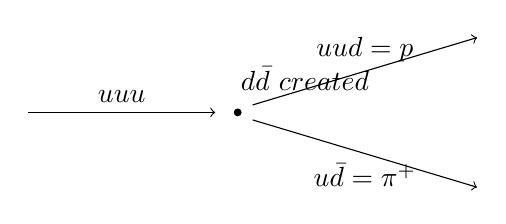
\begin{tikzpicture}[scale=0.95]
\draw[->] (-3,0) -- (-0.5,0) node[midway,above] {$uuu$};
\fill (-0.2,0) circle (1.5pt);
\draw[->] (0,0.1) -- (3,1.0) node[midway,above] {$uud=p$};
\draw[->] (0,-0.1) -- (3,-1.0) node[midway,below] {$u\bar d=\pi^+$};
\node at (0.7,0.45) {$d\bar d\ \text{created}$};
\end{tikzpicture}
\caption{Sự tái tổ hợp các thành phần trong phân rã \(\Delta^{++}\rightarrow p+\pi^+\).}
\end{figure}

Bảo toàn điện tích là điều thấy ngay:
\begin{equation}
Q(p)+Q(\pi^+)=1+1=2=Q(\Delta^{++}).
\end{equation}
Cân bằng khối lượng gần đúng cũng cho phép phân rã này:
\begin{equation}
1200\,\mathrm{MeV}
>
940\,\mathrm{MeV}+140\,\mathrm{MeV}.
\end{equation}
Còn đủ năng lượng cho động năng ở trạng thái cuối.

Cả bốn trạng thái Delta đều có thể phân rã thành proton hoặc neutron cùng với một pion. Thời gian sống của chúng cực kỳ ngắn. Một ước lượng bậc độ lớn là thời gian ánh sáng cần để đi qua một proton:
\begin{equation}
\tau_\Delta
\sim
\frac{10^{-13}\,\mathrm{cm}}
     {10^{10}\,\mathrm{cm/s}}
\sim10^{-23}\,\mathrm{s}.
\end{equation}
Tuy vậy, chúng vẫn sống đủ lâu để được nhận diện như những đối tượng riêng biệt được tạo ra trong các va chạm hạt.

\begin{classroomqa}
\audiencequestion{Thứ tự viết các ký hiệu \(u\) và \(d\) có quan trọng trong cách kiểm kê các thành phần này không?\lecturetimestamp{00:48:49}}
\lecturerresponse{Không, đối với mục đích đang xét. Thông tin quan trọng là nội dung hương và cách trạng thái lượng tử đầy đủ được kết hợp.}
\end{classroomqa}

\section{Câu đố Pauli và sự cần thiết của màu}

\(\Delta^{++}\) phơi bày một mâu thuẫn. Nó gồm ba quark up. Trong một trạng thái spin-\(\tfrac32\), các spin thông thường của chúng đều có thể cùng chỉ theo một hướng. Đẳng spin của chúng cũng đồng nhất vì tất cả đều là \(u\). Nếu spin, hương và trạng thái không gian năng lượng thấp nhất là toàn bộ mô tả, thì ba quark ấy sẽ là những fermion đồng nhất chiếm cùng một trạng thái. Nguyên lý loại trừ Pauli cấm điều này.

\begin{classroomqa}
\audiencequestion{Làm sao các quark up lặp lại ấy có thể là fermion nếu chúng dường như chiếm cùng một trạng thái?\lecturetimestamp{00:48:58}}
\lecturerresponse{Chúng không thể đồng nhất trong mọi số lượng tử. \(\Delta^{++}\) cho thấy quark cần một nhãn bổ sung ngoài spin thông thường, hương và trạng thái không gian. Nhãn bổ sung đó là màu.}
\end{classroomqa}

Nhãn mới này có ba giá trị khả dĩ:
\begin{equation}
r,\qquad g,\qquad b,
\end{equation}
được gọi là đỏ, lục và lam. Những từ này không liên quan gì đến màu sắc nhìn thấy được. Chúng là những tên gọi tùy ý cho ba trạng thái nội tại. Có thể đã dùng những tên khác; điều quan trọng là có ba khả năng phân biệt.

Phiên bản đỏ, lục và lam của một hương quark cho trước có cùng khối lượng và cùng các tính chất quan sát được thông thường. Tuy vậy, chúng vẫn là những trạng thái lượng tử khác nhau. Vì thế \(\Delta^{++}\) có thể chứa một \(u\) đỏ, một \(u\) lục và một \(u\) lam, nên ba fermion không chiếm cùng một trạng thái đầy đủ.

Sáu hương là
\begin{equation}
u,\ d,\ c,\ s,\ t,\ b.
\end{equation}
Thứ tự này không theo khối lượng. Quark up là nhẹ nhất và kế tiếp là quark down. Quark charm nặng hơn quark strange rất nhiều, và quark top nặng hơn quark bottom vượt trội. Mỗi hương có ba màu. Vì vậy, một quark mang ít nhất hai nhãn nội tại phân biệt:
\begin{equation}
\text{flavor}\quad\text{and}\quad\text{color}.
\end{equation}

Liệu thay vào đó ba quark có thể được phân biệt bằng vị trí hoặc động lượng không? Câu đố Delta liên quan đến trạng thái năng lượng thấp nhất, trong đó cấu trúc không gian và động lượng thích hợp không thể cung cấp ba nhãn phân biệt mà không làm thay đổi các tính chất năng lượng và đối xứng. Sự phân biệt còn thiếu phải là một bậc tự do nội tại mới.

Có một phép tương tự giàu ý nghĩa với vai trò của spin trong vật lý nguyên tử. Hai electron dường như chiếm cùng một trạng thái obitan vẫn có thể khác nhau bởi trạng thái spin của chúng. Theo cùng kiểu cấu trúc đó, các quark trùng nhau về hương, spin thông thường và trạng thái không gian vẫn có thể khác nhau về màu.

\editorialnote{Lộ trình lịch sử chính xác liên quan đến phổ helium, nguyên lý Pauli, và Uhlenbeck cùng Goudsmit đã được nêu rõ là chưa chắc chắn. Phép tương tự vẫn được giữ lại mà không khẳng định rằng đó là niên biểu chính xác theo đó spin đã được khám phá.}

Yoichiro Nambu được gắn với việc nhận ra rằng quark cần bậc tự do bổ sung này. Điểm vật lý là độc lập với tên gọi của nó: ba màu quark giải quyết mâu thuẫn Pauli. Nguyên lý loại trừ thích hợp ở đây là nguyên lý Pauli, không phải nguyên lý bất định Heisenberg.

\editorialnote{Việc quy công chính xác và lịch sử về sau của tên gọi \emph{color} đã được để ngỏ, nên ở đây không khẳng định một niên biểu chắc chắn hơn. Việc nhắc bằng lời đến nguyên lý bất định Heisenberg được sửa thành nguyên lý loại trừ Pauli, như lập luận xung quanh về thống kê fermion đòi hỏi.}

Cùng một cách xây dựng màu cũng áp dụng cho proton và neutron. Trạng thái của chúng không được dựng bằng cách gán một màu nhận dạng cố định cho từng ký hiệu hương được viết ra. Một baryon vật lý là chồng chập lượng tử của các cách gán đỏ, lục và lam có thể có, được kết hợp với các đối xứng trao đổi thích hợp.

\begin{classroomqa}
\audiencequestion{Màu có phải là một tính chất vật lý thông thường có thể đo trực tiếp không?\lecturetimestamp{00:56:55}}
\lecturerresponse{Ba màu có cùng khối lượng và cùng các tính chất thông thường. Sự khác biệt giữa chúng được bộc lộ theo quan hệ, thông qua các tổ hợp được phép và các quá trình va chạm. Thí nghiệm cho thấy có mặt ba trạng thái màu phân biệt, dù không thể chuẩn bị một quark mang màu cô lập để quan sát trực tiếp.}
\end{classroomqa}

\begin{classroomqa}
\audiencequestion{Màu có được bảo toàn không?\lecturetimestamp{00:57:38}}
\lecturerresponse{Có. Màu được bảo toàn, nhưng các hạt quan sát được đang bàn tới luôn có màu bằng không, nên đây là một định luật bảo toàn trông có phần khác thường.}
\end{classroomqa}

\editorialnote{Chính xác hơn, các hadron tiệm cận là các singlet màu. Cụm ``màu bằng không'' không phải là một điện tích tổng kiểu abel thu được bằng cách cộng số học đỏ, lục và lam.}

\begin{classroomqa}
\audiencequestion{Bản thân proton \(uud\) có thực sự cần cả ba màu không? Có vẻ chỉ cần phân biệt hai quark \(u\) là đủ.\lecturetimestamp{00:57:58}}
\lecturerresponse{Ví dụ đó hiển nhiên cần một sự phân biệt bổ sung nào đó, nhưng nó không khiến con số ba trở thành điều không thể tránh khỏi. \(\Delta^{++}\), với ba quark up có spin thông thường song song và đẳng spin song song, khiến nhu cầu về ba nhãn phân biệt trở nên không mơ hồ.}
\end{classroomqa}

Đó là lý do Delta đóng vai trò quan trọng đến vậy. Proton và neutron có các đối xứng spin và hương phức tạp hơn, nên mâu thuẫn có thể bị che khuất bởi các chi tiết của hàm sóng của chúng. Trong \(\Delta^{++}\), xung đột là tức thì:
\begin{equation}
uuu,\qquad
\uparrow\uparrow\uparrow,
\qquad
\text{one lowest spatial state}.
\end{equation}
Cần có một nhãn mới nhận ba giá trị. Sự tồn tại của ba trạng thái màu cũng được xác nhận độc lập bởi dữ liệu va chạm hadron.

Một nhãn đối xứng vẫn có thể có ý nghĩa ngay cả khi các lựa chọn của nó là tương đương khi tách riêng. Nếu không chọn một trục không gian, hai hướng spin là tương đương về mặt vật lý. Một đối tượng thứ hai có thể cung cấp một trục tham chiếu và bộc lộ quan hệ giữa chúng. Tương tự, proton hoặc neutron chọn ra một hướng trong không gian đẳng spin, và việc so sánh với các trạng thái khác cho thấy các định hướng nội tại là song song hay đối song song. Màu tinh tế hơn, nhưng nội dung vật lý của nó cũng xuất hiện thông qua các quan hệ, các tương quan và các quy tắc tương tác chứ không phải qua màu sắc nhìn thấy được.

Người ta cũng có thể tưởng tượng từ bỏ nguyên lý Pauli. Điều đó sẽ đòi hỏi một khuôn khổ toán học mới: lý thuyết trường lượng tử thông thường phân loại hạt thành fermion hoặc boson và không cung cấp một lựa chọn thứ ba đã được thiết lập nào giải quyết bài toán này. QCD giữ nguyên bản tính fermion của quark và đưa vào màu.

\begin{classroomqa}
\audiencequestion{Đại lượng quan sát nào tương ứng với sự phân biệt ẩn mà nguyên lý Pauli đòi hỏi?\lecturetimestamp{01:01:08}}
\lecturerresponse{Câu hỏi đó tinh tế hơn nhiều so với các đại lượng quan sát quen thuộc như vị trí, động lượng hay đẳng spin. Câu trả lời đầy đủ của nó đòi hỏi nhiều hơn về động lực học màu và được hoãn lại.}
\end{classroomqa}

\begin{classroomqa}
\audiencequestion{Tính chất fermion của quark có được suy ra từ các gán spin của hadron không?\lecturetimestamp{01:01:43}}
\lecturerresponse{Có.}
\end{classroomqa}

\editorialnote{Cách diễn đạt của hai câu hỏi trước đó từ cử tọa bị che khuất một phần. Chủ đề của chúng và các câu trả lời ngắn gọn là chắc chắn, nhưng không suy ra thêm một cách phát biểu chi tiết hơn.}

\begin{classroomqa}
\audiencequestion{Làm sao có thể gắn một màu cụ thể với một quark trong proton?\lecturetimestamp{01:01:55}}
\lecturerresponse{Người ta không gán một màu cố định cho một thành phần cấu thành có thể nhận dạng vĩnh viễn. Proton là một chồng chập lượng tử của mọi cách gán đỏ, lục và lam được phép, với các thừa số spin, hương, không gian và màu được đối xứng hóa hoặc phản đối xứng hóa một cách thích hợp. \(\Delta^{++}\) hữu ích vì cấu trúc spin và hương song song của nó phơi bày nhu cầu về màu mà không đòi hỏi hàm sóng proton đầy đủ.}
\end{classroomqa}

Đối với QCD, màu có vai trò giống như điện tích điện đối với điện động lực học: đó là số lượng tử chi phối tương tác. QCD mô tả dữ liệu thực nghiệm từ các va chạm hadron với độ chính xác rất cao. Sự biện minh sau cùng cho khuôn khổ này là các hệ quả của nó phù hợp với thực nghiệm.

\section{Photon và gluon}

Quark là các hạt vật chất fermion của QCD, tương tự electron trong QED ở phương diện hạn chế này. Điều gì liên kết chúng lại?

Trong điện động lực học, electron là một nguồn của trường điện từ. Theo ngôn ngữ hạt, nó phát ra và hấp thụ photon, và sự trao đổi photon tạo ra lực giữa các hạt mang điện. Tương tự, quark là một nguồn của trường gluon và có thể phát ra và hấp thụ gluon.

Gluon giống photon ở một số phương diện quan trọng. Chúng là những hạt spin 1 không khối lượng và có các trạng thái phân cực giống photon. Động lượng và phân cực của chúng là những tính chất động lực học thông thường. Khác biệt then chốt là gluon mang thông tin màu và vì thế tương tác với nhau.

Photon không mang điện tích. Ở mức sơ cấp của QED, một photon không phát ra một photon khác, và hai chùm sáng đi xuyên qua nhau mà không tương tác. Có những tương tác photon-photon bậc cao rất nhỏ có liên quan đến các vòng electron, nhưng đó là những hiệu ứng thứ cấp chứ không phải một sự tự ghép trực tiếp của photon. Trong không gian trống, đỉnh QED cơ bản đơn giản là electron phát ra hoặc hấp thụ một photon.

\begin{figure}[h]
\centering
\begin{tikzpicture}[scale=1.0]
\draw[->] (-2,-1) -- (0,0);
\draw[->] (0,0) -- (2,-1);
\draw[smooth] plot coordinates {
(0,0) (0.16,0.27) (0.32,0.23) (0.48,0.52)
(0.64,0.48) (0.80,0.77) (0.96,0.73)
(1.12,1.02) (1.28,0.98) (1.44,1.27)
(1.60,1.23) (1.76,1.52)
};
\node at (-1.25,-0.75) {$e^-$};
\node at (1.25,-0.75) {$e^-$};
\node at (1.95,1.62) {$\gamma$};
\fill (0,0) circle (1.5pt);
\end{tikzpicture}
\caption{Đỉnh QED cơ bản: electron phát ra hoặc hấp thụ một photon.}
\end{figure}

Đảo chiều của một đường fermion biến cách diễn giải như electron thành cách diễn giải như positron. Các quá trình phát xạ, hấp thụ và positron chéo đều chỉ là những cách sắp xếp lại của một đỉnh này.

Để tiện theo dõi, ta có thể giả vờ rằng photon có một số tính chất của một cặp electron--positron. Cặp này trung hòa điện, và spin của electron và positron khi thẳng hàng có thể tạo thành tổng spin bằng 1. Khi có một tương tác ngoài cung cấp năng lượng và động lượng cần thiết, photon có thể tạo ra một cặp electron--positron. Không điều nào trong số này có nghĩa là photon theo nghĩa đen được tạo thành từ một electron và một positron. Bức tranh cặp giả định đó đóng góp rất ít cho chính QED, nhưng phép tương tự màu của nó lại hữu ích trong QCD.

\section{Các nhãn màu--phản màu của gluon}

Biểu diễn ba trạng thái màu của một quark dưới dạng một cột:
\begin{equation}
q=
\begin{pmatrix}
r\\
g\\
b
\end{pmatrix}.
\end{equation}
Biểu diễn các nhãn phản quark tương ứng dưới dạng một hàng:
\begin{equation}
\bar q=
\begin{pmatrix}
\bar r&\bar g&\bar b
\end{pmatrix}.
\end{equation}

Gluon không phải là một trạng thái liên kết quark--phản quark. Tuy vậy, về mặt hạch toán màu, nó ứng xử như thể mang một màu và một phản màu. Vì thế, các nhãn khả dĩ có thể được sắp thành
\begin{equation}
\begin{pmatrix}
r\bar r&r\bar g&r\bar b\\
g\bar r&g\bar g&g\bar b\\
b\bar r&b\bar g&b\bar b
\end{pmatrix}.
\end{equation}
Thoạt nhìn, điều này cho 9 tổ hợp.

\begin{classroomqa}
\audiencequestion{Các phần tử đường chéo màu--phản màu có không phân biệt được với nhau không?\lecturetimestamp{01:13:37}}
\lecturerresponse{Không đơn giản như vậy. Các phần tử đường chéo là phân biệt; điểm mấu chốt là tổng của chúng không phải là một trạng thái lượng tử độc lập.}
\end{classroomqa}

Thực ra chỉ có 8 trạng thái gluon độc lập. Ba nhãn đường chéo không đơn giản là không phân biệt được với nhau, nhưng tổng đường chéo riêng biệt
\begin{equation}
r\bar r+g\bar g+b\bar b
\end{equation}
không tạo ra thêm một gluon độc lập nào của QCD. Lời giải thích sâu hơn cho sự rút gọn này sẽ được hoãn lại. Đối với các lập luận về dòng màu hiện tại, sẽ hữu ích nếu làm việc với 9 nhãn bề ngoài và nhớ rằng thiếu một tổ hợp đường chéo.

\section{Đỉnh quark--gluon}

Một quark có thể phát ra một gluon và đi ra với màu giữ nguyên hoặc thay đổi. Nếu một quark đi vào với màu \(a\) và đi ra với màu \(b\), gluon được phát ra mang nhãn hạch toán \(a\bar b\):
\begin{equation}
a\longrightarrow b+(a\bar b).
\end{equation}
Ví dụ,
\begin{equation}
r\longrightarrow g+(r\bar g).
\end{equation}
Đường màu đỏ tiếp tục đi vào gluon, còn đường màu lục tiếp tục qua quark đi ra và đảo chiều thành một đường phản lục trong gluon.

Quark không nhất thiết phải đổi màu. Cùng quy tắc ấy cũng cho phép
\begin{equation}
r\longrightarrow r+(r\bar r),
\end{equation}
hoặc
\begin{equation}
r\longrightarrow b+(r\bar b).
\end{equation}

\begin{figure}[h]
\centering
\begin{tikzpicture}[scale=1.0]
\draw[->] (-2,-0.8) -- (0,0) node[midway,above] {$r$};
\draw[->] (0,0) -- (2,0.9) node[midway,above] {$g$};
\draw[smooth] plot coordinates {
(0,0) (0.20,-0.23) (0.40,-0.17) (0.60,-0.46)
(0.80,-0.40) (1.00,-0.69) (1.20,-0.63)
(1.40,-0.92) (1.60,-0.86) (1.80,-1.15)
(2.00,-1.09)
};
\node at (2.35,-1.12) {$r\bar g$};
\fill (0,0) circle (1.5pt);
\end{tikzpicture}
\caption{Một quark đỏ trở thành quark lục đồng thời phát ra một gluon \(r\bar g\).}
\end{figure}

Đây là một viên gạch tương tác sơ cấp của QCD.

\begin{classroomqa}
\audiencequestion{Có phải gluon chỉ có thể được phát ra khi quark đổi màu không?\lecturetimestamp{01:17:15}}
\lecturerresponse{Không. Quark đi ra có thể có cùng màu hoặc màu khác. Trong cả hai trường hợp, nhãn màu--phản màu của gluon phát ra làm cho các đường màu liên tục.}
\end{classroomqa}

\section{Đỉnh ba gluon}

QCD còn có một tương tác sơ cấp khác không có đối ứng cơ bản trong QED. Một gluon có thể tương tác trực tiếp với các gluon khác.

Bắt đầu với một gluon \(r\bar b\). Theo ngôn ngữ dòng màu, nó có thể tách thành
\begin{equation}
r\bar b
\longrightarrow
r\bar g+g\bar b.
\end{equation}
Đường đỏ tiếp tục vào \(r\bar g\), đường phản lam tiếp tục vào \(g\bar b\), và cặp lục-phản lục nối hai gluon đi ra. Điều này cho ta một đỉnh ba gluon.

\begin{figure}[h]
\centering
\begin{tikzpicture}[scale=1.0]
\draw[smooth] plot coordinates {
(-2,0) (-1.80,0.12) (-1.60,-0.02) (-1.40,0.12)
(-1.20,-0.02) (-1.00,0.12) (-0.80,-0.02)
(-0.60,0.12) (-0.40,-0.02) (-0.20,0.12) (0,0)
};
\draw[smooth] plot coordinates {
(0,0) (0.20,0.27) (0.40,0.21) (0.60,0.50)
(0.80,0.44) (1.00,0.73) (1.20,0.67)
(1.40,0.96) (1.60,0.90) (1.80,1.19) (2.00,1.13)
};
\draw[smooth] plot coordinates {
(0,0) (0.20,-0.27) (0.40,-0.21) (0.60,-0.50)
(0.80,-0.44) (1.00,-0.73) (1.20,-0.67)
(1.40,-0.96) (1.60,-0.90) (1.80,-1.19) (2.00,-1.13)
};
\node at (-2.45,0) {$r\bar b$};
\node at (2.45,1.18) {$r\bar g$};
\node at (2.45,-1.18) {$g\bar b$};
\fill (0,0) circle (1.5pt);
\end{tikzpicture}
\caption{Dòng màu ba gluon: \(r\bar b\rightarrow r\bar g+g\bar b\).}
\end{figure}

Không cần phải ghi nhớ mọi tổ hợp được phép. Hãy lần theo từng đường màu xuyên suốt giản đồ. Khi một đường fermion đảo hướng theo thời gian, hãy diễn giải lại nó như đường phản hạt hoặc phản màu tương ứng.

\section{Trao đổi gluon và các lực}

Gluon tạo ra lực bằng cách được trao đổi, đúng như photon tạo ra lực điện từ bằng cách được trao đổi giữa các hạt mang điện.

Ví dụ, một quark lam và một phản quark phản lam có thể trao đổi một gluon \(g\bar b\) và đi ra thành lục và phản lục. Một cách gán dòng màu thỏa mãn cả hai đỉnh là\footnote{Sự đổi màu tổng thể \(b+\bar b\longrightarrow g+\bar g\) là tường minh, nhưng các nhãn màu cục bộ được hiệu chỉnh nhiều lần. Nhãn trao đổi \(g\bar b\) được dựng lại bằng cách đòi hỏi dòng màu liên tục tại cả hai đỉnh.}
\begin{equation}
b+\bar b
\longrightarrow
g+\bar g.
\end{equation}
Tại đỉnh phản quark,
\begin{equation}
\bar b\longrightarrow\bar g+(g\bar b),
\end{equation}
còn tại đỉnh quark,
\begin{equation}
b+(g\bar b)\longrightarrow g.
\end{equation}
Gluon trao đổi mang sự thay đổi màu từ đường fermion này sang đường fermion kia.

\begin{figure}[h]
\centering
\begin{tikzpicture}[scale=1.0]
\draw[->] (-1.8,0) -- (-1.8,-1.8) node[midway,left] {$\bar b$};
\draw[->] (-1.8,1.8) -- (-1.8,0) node[midway,left] {$\bar g$};
\draw[->] (1.8,-1.8) -- (1.8,0) node[midway,right] {$b$};
\draw[->] (1.8,0) -- (1.8,1.8) node[midway,right] {$g$};
\draw[smooth] plot coordinates {
(-1.8,0) (-1.50,0.13) (-1.20,-0.03) (-0.90,0.13)
(-0.60,-0.03) (-0.30,0.13) (0,-0.03)
(0.30,0.13) (0.60,-0.03) (0.90,0.13)
(1.20,-0.03) (1.50,0.13) (1.8,0)
};
\node at (0,0.42) {$g\bar b$};
\fill (-1.8,0) circle (1.5pt);
\fill (1.8,0) circle (1.5pt);
\end{tikzpicture}
\caption{Sự trao đổi một gluon \(g\bar b\) biến một cặp lam--phản lam thành một cặp lục--phản lục; các mũi tên của phản quark hướng ngược với chiều thời gian tăng.}
\end{figure}

Cùng tương tác ấy cũng cho phép có lực giữa các gluon. Một cách thể hiện nhất quán là\footnote{Bài giảng xác lập sự trao đổi gluon giữa các gluon và quy tắc lần theo các đường, nhưng các nhãn cục bộ trong giản đồ được sửa đi sửa lại nhiều lần. Cách gán được hiển thị là một cách thể hiện nhất quán của quy tắc cuối cùng, chứ không phải một bản chép chắc chắn của mọi nhãn trung gian.}
\begin{equation}
(r\bar b)+(b\bar r)
\longrightarrow
(r\bar g)+(g\bar r),
\end{equation}
với một gluon \(g\bar b\) được trao đổi giữa hai gluon ngoài:
\begin{align}
r\bar b&\longrightarrow r\bar g+g\bar b,\\
b\bar r+g\bar b&\longrightarrow g\bar r.
\end{align}

\begin{figure}[h]
\centering
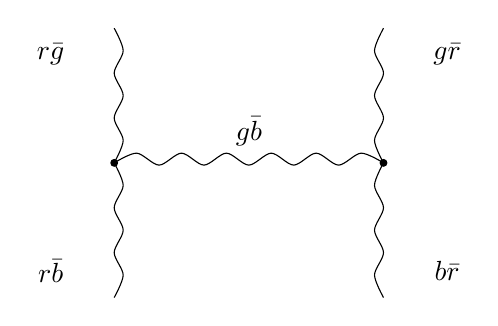
\begin{tikzpicture}[scale=0.95]
\draw[smooth] plot coordinates {
(-1.8,-1.8) (-1.68,-1.50) (-1.80,-1.20) (-1.68,-0.90)
(-1.80,-0.60) (-1.68,-0.30) (-1.8,0)
};
\draw[smooth] plot coordinates {
(-1.8,0) (-1.68,0.30) (-1.80,0.60) (-1.68,0.90)
(-1.80,1.20) (-1.68,1.50) (-1.8,1.8)
};
\draw[smooth] plot coordinates {
(1.8,-1.8) (1.68,-1.50) (1.80,-1.20) (1.68,-0.90)
(1.80,-0.60) (1.68,-0.30) (1.8,0)
};
\draw[smooth] plot coordinates {
(1.8,0) (1.68,0.30) (1.80,0.60) (1.68,0.90)
(1.80,1.20) (1.68,1.50) (1.8,1.8)
};
\draw[smooth] plot coordinates {
(-1.8,0) (-1.50,0.13) (-1.20,-0.03) (-0.90,0.13)
(-0.60,-0.03) (-0.30,0.13) (0,-0.03)
(0.30,0.13) (0.60,-0.03) (0.90,0.13)
(1.20,-0.03) (1.50,0.13) (1.8,0)
};
\node at (-2.65,-1.45) {$r\bar b$};
\node at (-2.65,1.45) {$r\bar g$};
\node at (2.65,-1.45) {$b\bar r$};
\node at (2.65,1.45) {$g\bar r$};
\node at (0,0.42) {$g\bar b$};
\fill (-1.8,0) circle (1.5pt);
\fill (1.8,0) circle (1.5pt);
\end{tikzpicture}
\caption{Sự trao đổi một gluon \(g\bar b\) giữa hai gluon, với mỗi đường màu và phản màu đều liên tục qua các đỉnh.}
\end{figure}

\section{Tự tương tác gluon và các trường phi tuyến}

Tự tương tác của gluon làm thay đổi bản chất của QCD. Quark có thể liên kết với nhau bằng trao đổi gluon và tạo thành hadron, nhưng gluon cũng có thể liên kết với nhau bằng trao đổi gluon. Vì vậy QCD có thể chứa các đối tượng hợp thành được tạo nên hoàn toàn từ các bậc tự do gluon, không có quark. Trong QED không có trạng thái liên kết tương ứng nào ở mức sơ cấp chỉ được tạo bởi photon.

Ngôn ngữ trường cho cùng một kết luận. Hai sóng điện từ trong không gian trống đi xuyên qua nhau ở mức sơ cấp. Hai sóng gluon thì tương tác và làm biến dạng lẫn nhau. Ngay cả các phần khác nhau của một cấu hình trường gluon cũng có thể tác dụng lực lên nhau. Vì vậy trường gluon là phi tuyến.

\begin{classroomqa}
\audiencequestion{Có phải ở mỗi phía của một giản đồ phải xuất hiện cùng số lượng các nhãn đỏ, lục và lam không?\lecturetimestamp{01:24:59}}
\lecturerresponse{Quy tắc thực hành là lần theo mọi đường màu xuyên suốt giản đồ. Sự liên tục đó chính là bảo toàn màu. Nếu một đường fermion quay ngược lại theo thời gian, nhãn của nó trở thành nhãn phản hạt hoặc phản màu tương ứng.}
\end{classroomqa}

\begin{classroomqa}
\audiencequestion{Có phải mọi nhãn màu và phản màu trong phiên bản đầu của giản đồ đều nhất quán không?\lecturetimestamp{01:26:00}}
\lecturerresponse{Không. Một số nhãn phải được hiệu chỉnh. Trong một cách gán nhất quán, các đường đỏ, phản lam và lục mỗi đường đều tiếp tục qua các đỉnh, với mũi tên fermion bị đảo được diễn giải là một phản hạt.}
\end{classroomqa}

\begin{classroomqa}
\audiencequestion{Có phải một đường gluon trung gian đang được xem như một cặp quark--phản quark không?\lecturetimestamp{01:27:58}}
\lecturerresponse{Chỉ trong việc hạch toán màu của nó. Gluon theo nghĩa đen không phải là một hợp thể quark--phản quark, nhưng nó mang các tính chất màu và phản màu tương ứng.}
\end{classroomqa}

Ở giai đoạn này, các quy tắc cơ bản có thể tóm gọn như sau:

\begin{itemize}
\item quark phát ra và hấp thụ gluon;
\item gluon tương tác trực tiếp với gluon;
\item mọi đường màu và phản màu đều phải tiếp tục qua một đỉnh;
\item đảo chiều theo thời gian của một đường fermion biến nó thành đường phản hạt tương ứng.
\end{itemize}

\begin{classroomqa}
\audiencequestion{Khi được biểu diễn bằng tất cả những đường màu--phản màu này, gluon vẫn không khối lượng chứ?\lecturetimestamp{01:28:13}}
\lecturerresponse{Có. Gluon vẫn không khối lượng. Phần lưu ý sau đây liên quan đến ý nghĩa của khối lượng được gán cho một quark bên trong hadron.}
\end{classroomqa}

Tiếp theo là giam cầm và cấu trúc của hadron: vì sao màu cô lập không bao giờ được quan sát thấy và quark cùng gluon tự tổ chức như thế nào bên trong các hạt hợp thành. Trước hết, sẽ hữu ích nếu làm rõ điều được hiểu là khối lượng của một quark thành phần.

\section{Thang thăm dò và ý nghĩa của khối lượng quark}

Hãy hình dung một vật nhỏ có khối lượng \(m\) gắn với một mẩu vật liệu mềm, dễ biến dạng---một mẩu kẹo cao su thõng xuống là đủ. Tác dụng một lực thật nhẹ, chậm đến mức vật liệu mềm có thời gian điều chỉnh và toàn bộ hệ chuyển động cùng nhau. Khi đó quán tính đo được là quán tính của vật nhỏ cộng với phần vật liệu gắn kèm.

Bây giờ hãy làm rung vật nhỏ ấy ở tần số rất cao. Vật liệu mềm không có thời gian để theo kịp chuyển động nhanh. Nó gần như đứng yên trong khi lõi nhỏ đáp ứng. Khi đó quán tính đo được ở tần số cao gần với riêng \(m\) hơn nhiều.

\begin{figure}[h]
\centering
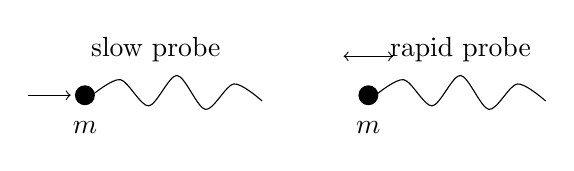
\begin{tikzpicture}[scale=0.9]
\fill (-3,0) circle (4pt);
\node at (-3,-0.45) {$m$};
\draw[smooth] plot coordinates {
(-2.9,0) (-2.5,0.22) (-2.1,-0.15) (-1.7,0.28)
(-1.3,-0.20) (-0.9,0.16) (-0.5,-0.08)
};
\draw[->] (-3.8,0) -- (-3.2,0);
\node at (-2.0,0.65) {slow probe};

\fill (1.0,0) circle (4pt);
\node at (1.0,-0.45) {$m$};
\draw[smooth] plot coordinates {
(1.1,0) (1.5,0.22) (1.9,-0.15) (2.3,0.28)
(2.7,-0.20) (3.1,0.16) (3.5,-0.08)
};
\draw[<->] (0.65,0.55) -- (1.35,0.55);
\node at (2.3,0.65) {rapid probe};
\end{tikzpicture}
\caption{Một phép thăm dò chậm làm lõi và phần gắn mềm của nó chuyển động cùng nhau, còn một phép thăm dò nhanh ban đầu chủ yếu đo đáp ứng của lõi.}
\end{figure}

Đây là một phép tương tự cổ điển. Khối lượng được suy ra phụ thuộc vào tần số của lực tác dụng vì các phần khác nhau của hệ có thời gian tham gia ở những tần số khác nhau.

Một quark bên trong hadron được bao quanh bởi vật chất gluon tương tác mạnh và bởi các thành phần cấu tạo khác. Nếu có thể kéo rất chậm lên một quark, toàn bộ hadron sẽ đáp ứng. Khi đó quán tính gặp phải sẽ có bậc cỡ khối lượng nucleon,
\begin{equation}
m_N\sim930\text{--}940\,\mathrm{MeV}.
\end{equation}
Nếu quark bị đánh rất mạnh và được thăm dò trong một khoảng thời gian rất ngắn, thì đáp ứng ban đầu gắn với tham số khối lượng nhỏ hơn rất nhiều vốn theo quy ước được gán cho một quark nhẹ, xấp xỉ
\begin{equation}
m_{u,d}\sim5\text{--}10\,\mathrm{MeV}
\end{equation}
trong các ước lượng đang được dùng ở đây.

Vì vậy, cụm từ ``khối lượng của một quark'' đòi hỏi phải chỉ rõ thang của phép thăm dò. Một nhiễu loạn nhẹ, tần số thấp làm chuyển động toàn bộ hợp thể mở rộng; một nhiễu loạn mạnh, tần số cao ban đầu phân giải một phần nhỏ hơn nhiều của nó. Phép tương tự này không phải là một suy dẫn của sự tái chuẩn hóa, nhưng nó gợi ra vì sao các tham số dùng để mô tả hạt lại phụ thuộc vào các tần số và bước sóng của những tương tác trong đó chúng được đo. Những tham số phụ thuộc thang như vậy được gọi là các tham số chạy hoặc các hằng số chạy.

\begin{classroomqa}
\audiencequestion{Khối lượng phụ thuộc tần số này có chỉ đơn thuần là một cách phát biểu lại của một hệ thức bất định như \(\Delta x\,\Delta t\) không?\lecturetimestamp{01:33:32}}
\lecturerresponse{Không. Ví dụ này đã là một hiện tượng cổ điển rồi. Một khối lượng nhỏ gắn với một thứ mềm sẽ gia tốc theo một cách dưới tác dụng của lực nhanh và theo một cách khác dưới tác dụng của lực chậm, vì những lượng khác nhau của phần vật liệu gắn kèm có thời gian để đáp ứng.}
\end{classroomqa}

\begin{classroomqa}
\audiencequestion{Phần thảo luận trước đó về điện tích của electron có liên quan đến cùng kiểu phụ thuộc thang này không?\lecturetimestamp{01:34:04}}
\lecturerresponse{Có. Bài học tổng quát là các tham số dùng để mô tả hạt phụ thuộc vào các tần số và bước sóng của những tương tác dùng để thăm dò chúng. Chúng được gọi là các hằng số chạy.}
\end{classroomqa}

\begin{classroomqa}
\audiencequestion{Điều bảo lưu tương tự có áp dụng cho điện tích phân số được gán cho một quark không?\lecturetimestamp{01:34:36}}
\lecturerresponse{Có. Ta phải định nghĩa cẩn thận điều được hiểu là điện tích của một quark. Ở mức này, nó được nêu tương đối so với điện tích proton; một định nghĩa đầy đủ hơn thuộc về một thảo luận riêng.}
\end{classroomqa}

\editorialnote{Số lượng tử điện tích phân số cố định và hằng số ghép tương tác phụ thuộc vào thang là những đại lượng phân biệt. Sự chạy của hằng số ghép không làm thay đổi chính các nhãn hương vị \(+\tfrac23\) hay \(-\tfrac13\).}

\begin{classroomqa}
\audiencequestion{Tại sao việc xét màu luôn dùng một quark và một phản quark? Vì sao hai quark lại không thể tạo thành đối tượng tương ứng?\lecturetimestamp{01:34:55}}
\lecturerresponse{Đó là một câu hỏi quan trọng, nhưng câu trả lời thuộc về phần thảo luận tiếp theo về các tổ hợp màu được phép và sự giam hãm.}
\end{classroomqa}

\begin{classroomqa}
\audiencequestion{Nếu các quark riêng lẻ không thể được cô lập, thì điện tích phân số, màu và mô hình quark đã được suy ra như thế nào?\lecturetimestamp{01:35:17}}
\lecturerresponse{Bức tranh đó dần dần hiện ra từ nhiều manh mối cùng với những mâu thuẫn biểu kiến. Các mẫu hình hadron gợi ý các thành phần quark; các trạng thái Delta làm lộ ra một xung đột với thống kê Fermi; và sự giam hãm vĩnh viễn của quark cung cấp thêm một sự kiện kỳ lạ khác. Đề xuất về quark xuất hiện vào đầu những năm 1960, Nambu đã có một phiên bản sớm quan trọng của ý tưởng màu, và nhiều nhà vật lý đã xây dựng và kiểm nghiệm toàn bộ cấu trúc ấy trong khoảng thập niên tiếp theo. Đó không phải là kết quả của một quan sát duy nhất hay của một cá nhân duy nhất.}
\end{classroomqa}

\begin{classroomqa}
\audiencequestion{Tại sao chỉ có tám gluon thay vì chín tổ hợp màu--phản màu có vẻ như có thể có?\lecturetimestamp{01:37:24}}
\lecturerresponse{Lời giải thích chi tiết về việc vì sao tổng theo đường chéo không phải là một gluon bổ sung được hoãn lại.}
\end{classroomqa}

\begin{classroomqa}
\audiencequestion{Phần thảo luận này về QCD có đang bỏ qua electron không?\lecturetimestamp{01:37:33}}
\lecturerresponse{Có. QCD đang được tách riêng ra theo cùng cách mà một phần thảo luận về QED có thể tạm thời bỏ qua quark. Cuối cùng, các sector riêng biệt phải được kết hợp thành một cấu trúc lớn hơn chứa quark, electron, photon và các hạt khác. Một số phần của sự tổng hợp lớn hơn đó đã được hoàn thành, và một số phần vẫn còn chưa hoàn chỉnh. Vật lý thường tiến triển bằng cách tách riêng một hệ con, hiểu nó, rồi ghép các mảnh lại với nhau.}
\end{classroomqa}